%%%%%%%%%%%%%%%%%%%%%%%%%%%%%%%%%%%%%%%%%%%%%%%%%%%%%%%%%%%%%%%%%%%%%%%%%%%%%%%%%%%%%%%%%%%%
%%
%% Chapter 2 : Background
%%
%%      * Should give the necessary info/math/tools to understand the proposal
%%
%%  BASIC STRUCTURE :
%%
%%      a. DRL overview
%%            * RL overview
%%            * RL methods
%%            * Policy Optimization
%%            * Deep Learning and RL
%%
%%      b. Simulated environments (talk about ALE, Gym)
%%
%%      c. Simulated environments for robot locomotion
%%          * Physics engines
%%          * Kinematic trees
%%          * Actuation models
%%
%%%%%%%%%%%%%%%%%%%%%%%%%%%%%%%%%%%%%%%%%%%%%%%%%%%%%%%%%%%%%%%%%%%%%%%%%%%%%%%%%%%%%%%%%%%%
\chapter{Background}
\label{ch:background}

%%%%%%%%%%%%%%%%%%%%%%%%%%%%%%%
%   Figures for chapter 2
%%%%%%%%%%%%%%%%%%%%%%%%%%%%%%%

\newcommand{\figrlloop}{
    \begin{figure}
        \centering
        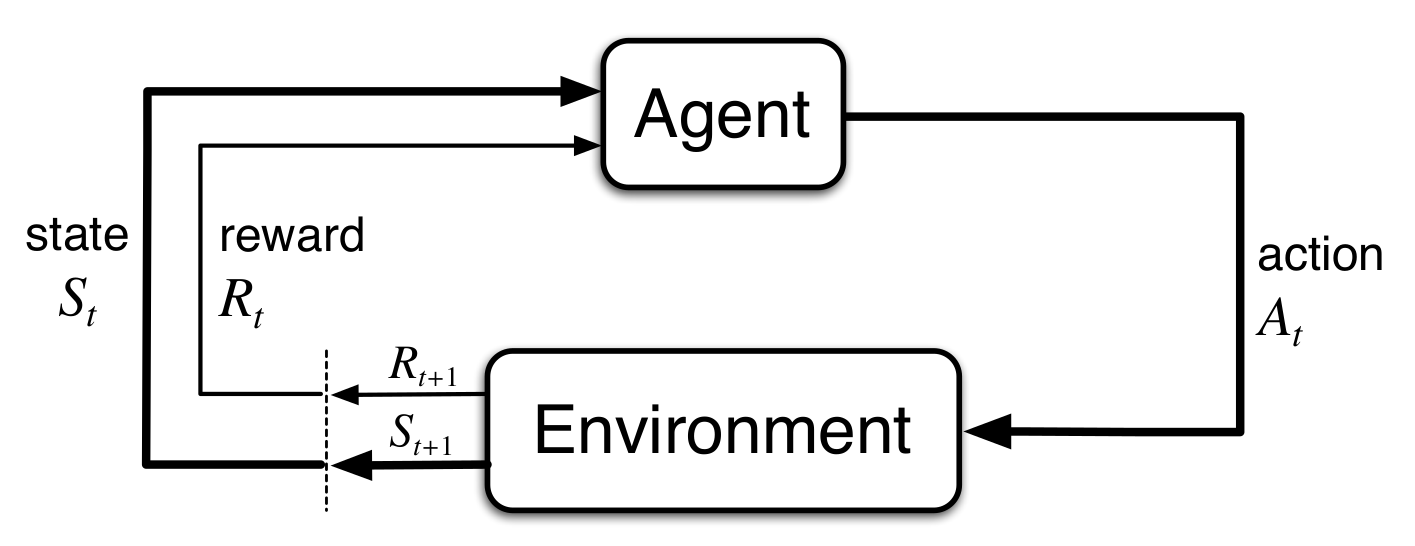
\includegraphics[width=5in]{./chapters/chapter_2/imgs/img_rl_loop.png}
        \caption{Agent-Environment interaction loop}
        \label{fig:ch2_rlloop}
    \end{figure}
}

\newcommand{\figdrlsamplesFirst}{
    \begin{figure}
        \centering
        \begin{subfigure}[b]{0.4\textwidth}
            \centering
            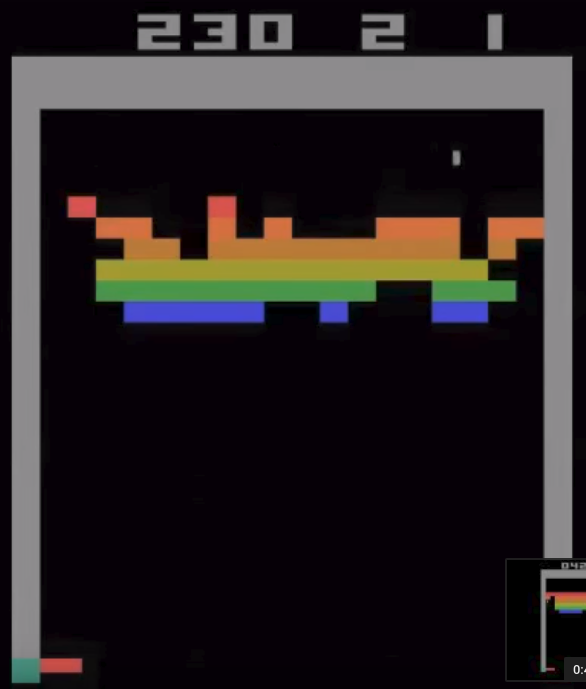
\includegraphics[width=0.9\textwidth]{./chapters/chapter_2/imgs/img_dqn_breakout.png}
            \caption{}
            \label{fig:ch2_dqn_breakout}
        \end{subfigure}
        \begin{subfigure}[b]{0.4\textwidth}
            \centering
            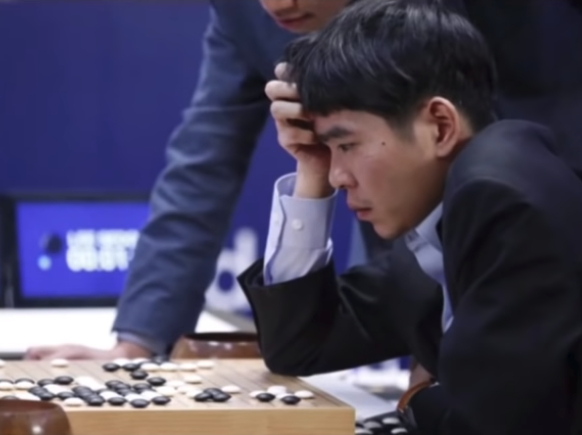
\includegraphics[width=0.9\textwidth]{./chapters/chapter_2/imgs/img_alphago.png}
            \caption{}
            \label{fig:ch2_alphago}
        \end{subfigure}
        \caption{Some DeepRL success stories: (a) DQN agent playing atari breakout [@CITE],
                                              (b) AlphaGo playing against Go champion Lee Sedol [@CITE]}
        \label{fig:ch2_drl_stories_1}
    \end{figure}
}

\newcommand{\figdrlsamplesSecond}{
    \begin{figure}
        \centering
        \begin{subfigure}[b]{0.3\textwidth}
            \centering
            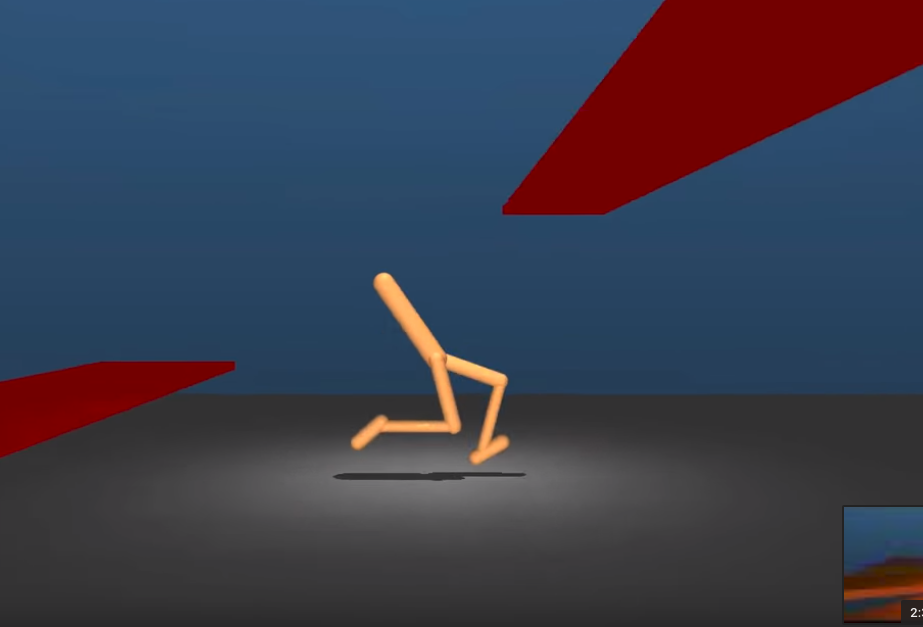
\includegraphics[width=0.9\textwidth]{./chapters/chapter_2/imgs/img_emergence_of_locomotion.png}
            \caption{}
            \label{fig:ch2_emergence_of_locomotion}
        \end{subfigure}
        \begin{subfigure}[b]{0.3\textwidth}
            \centering
            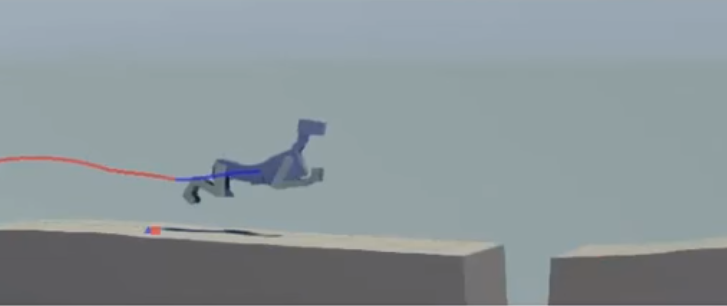
\includegraphics[width=0.9\textwidth]{./chapters/chapter_2/imgs/img_deepterrainrl.png}
            \caption{}
            \label{fig:ch2_deepterrainrl}
        \end{subfigure}
        \begin{subfigure}[b]{0.3\textwidth}
            \centering
            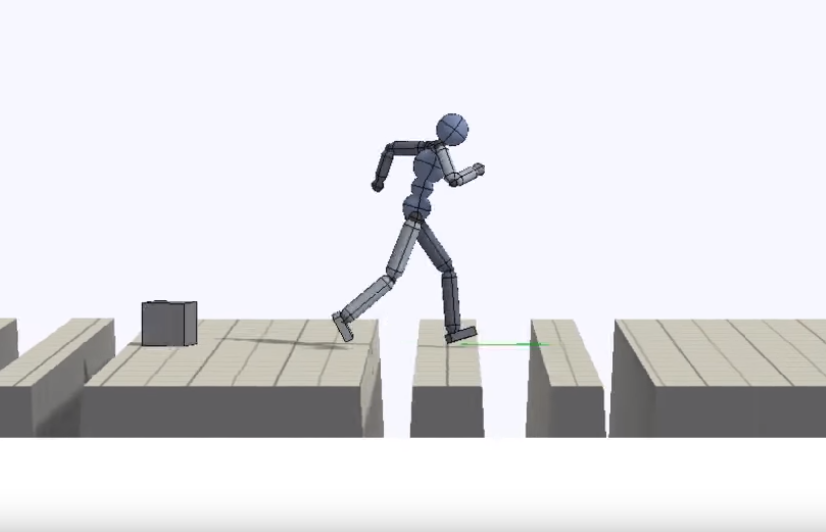
\includegraphics[width=0.9\textwidth]{./chapters/chapter_2/imgs/img_deepmimic.png}
            \caption{}
            \label{fig:ch2_deepmimic}
        \end{subfigure}
        \caption{Some DeepRL success stories: (a) Deepmind's agent running in a simulated environment [@CITE],
                                              (b) Simulated dog running in a course with obstacles [@CITE],
                                              (c) Simulated character running in an obstacle course, while 
                                                  mimicking humans' natural motion [@CITE]}
        \label{fig:ch2_drl_stories_2}
    \end{figure}
}

\newcommand{\figdrlsamplesThird}{
    \begin{figure}
        \centering
        \begin{subfigure}[b]{0.3\textwidth}
            \centering
            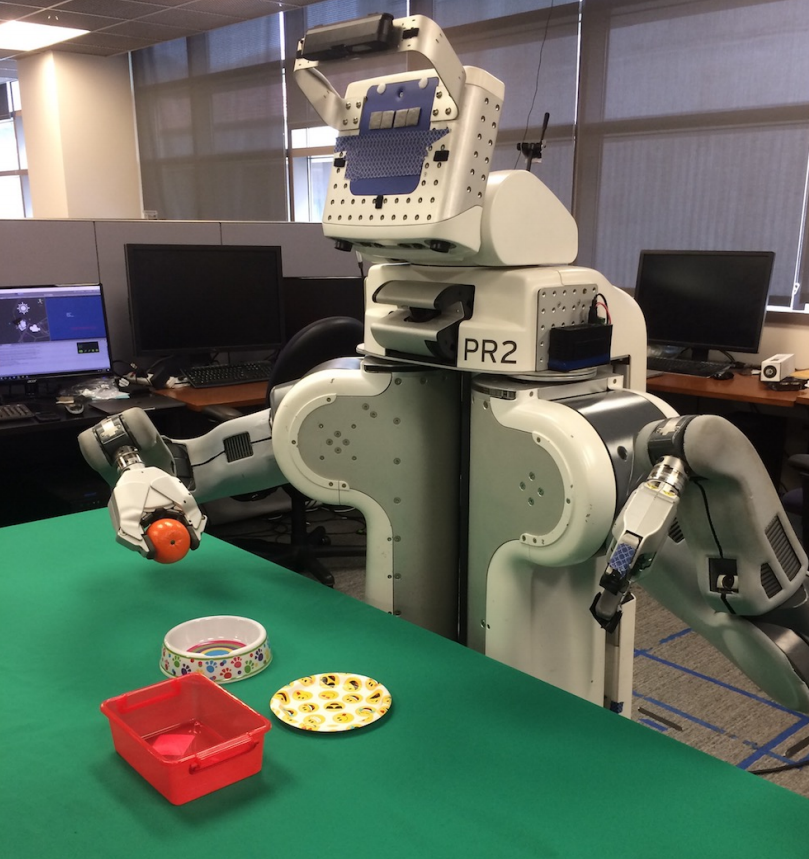
\includegraphics[width=0.9\textwidth]{./chapters/chapter_2/imgs/img_visual_motor_control.png}
            \caption{}
            \label{fig:ch2_visual_motor_control}
        \end{subfigure}
        \begin{subfigure}[b]{0.3\textwidth}
            \centering
            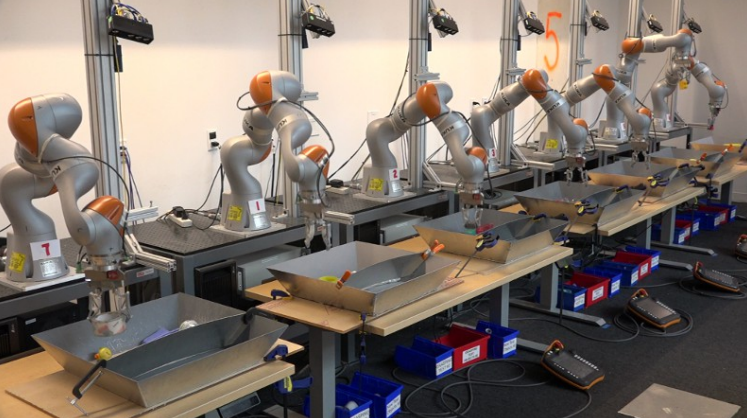
\includegraphics[width=0.9\textwidth]{./chapters/chapter_2/imgs/img_vision_based_robotics.png}
            \caption{}
            \label{fig:ch2_vision_based_robotics}
        \end{subfigure}
        \begin{subfigure}[b]{0.3\textwidth}
            \centering
            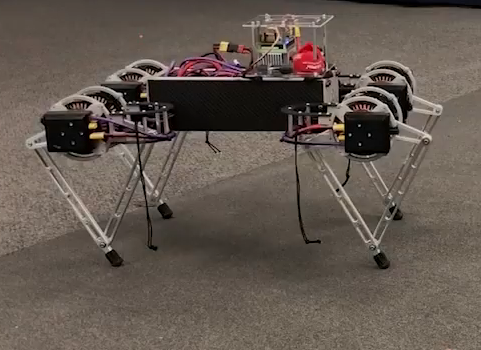
\includegraphics[width=0.9\textwidth]{./chapters/chapter_2/imgs/img_sim_2_real.png}
            \caption{}
            \label{fig:ch2_sim_2_real}
        \end{subfigure}
        \caption{Some DeepRL success stories: (a) PR2 robot learning manipulation tasks [@CITE],
                                              (b) Learning more manipulation tasks using lots of robots [@CITE],
                                              (c) Quadruped running in the real world [@CITE]}
        \label{fig:ch2_drl_stories_3}
    \end{figure}
}

\newcommand{\figMdpSamples}{
    \begin{figure}
        \centering
        \begin{subfigure}[b]{0.9\textwidth}
            \centering
            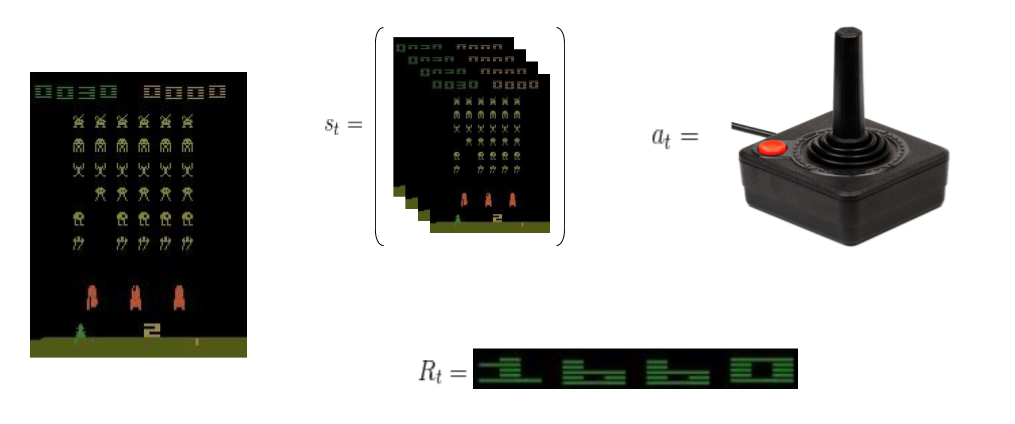
\includegraphics[width=0.9\textwidth]{./chapters/chapter_2/imgs/img_rl_mdp_atari.png}
            \caption{}
            \label{fig:ch2_mdp_sample_atari}
        \end{subfigure}

        \centering
        \begin{subfigure}[b]{0.9\textwidth}
            \centering
            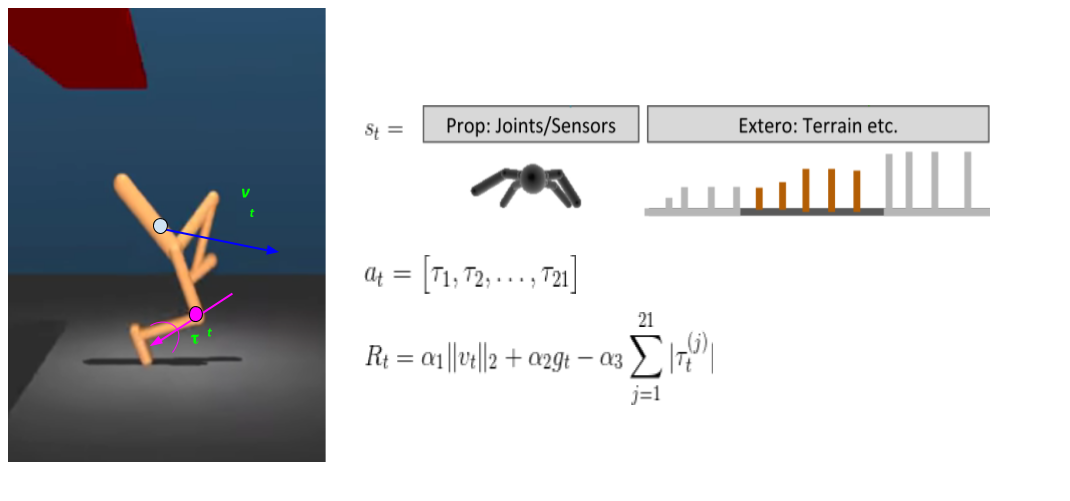
\includegraphics[width=0.9\textwidth]{./chapters/chapter_2/imgs/img_rl_mdp_locomotion.png}
            \caption{}
            \label{fig:ch2_mdp_sample_locomotion}
        \end{subfigure}
        \caption{Some examples of MDPs: (a) MDP modelling an Atari game. 
                                        (b) MDP modelling a locomotion task.}
        \label{fig:ch2_mdps_samples}
    \end{figure}
}

\newcommand{\figRlPolicies}{
    \begin{figure}
        \centering
        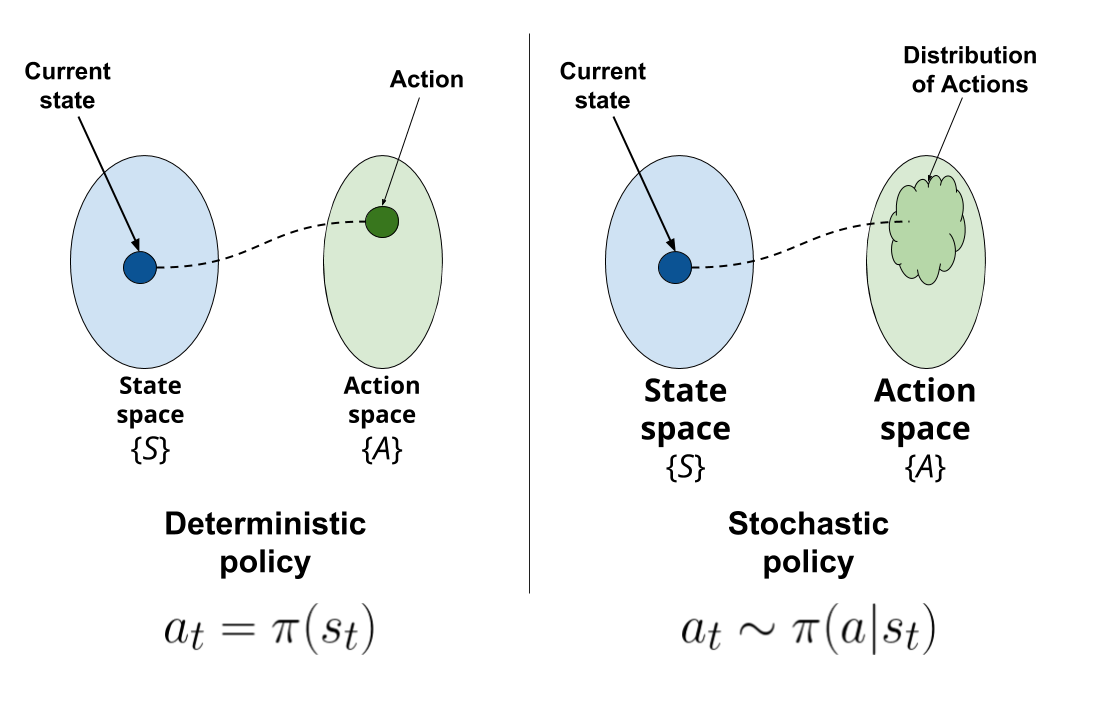
\includegraphics[width=0.9\textwidth]{./chapters/chapter_2/imgs/img_rl_policies.png}
        \caption{Differences between deterministic and stochastic policies.}
        \label{fig:ch2_rl_policies_differences}
    \end{figure}
}

\newcommand{\figRlMethodsLandspace}{
    \begin{figure}
        \centering
        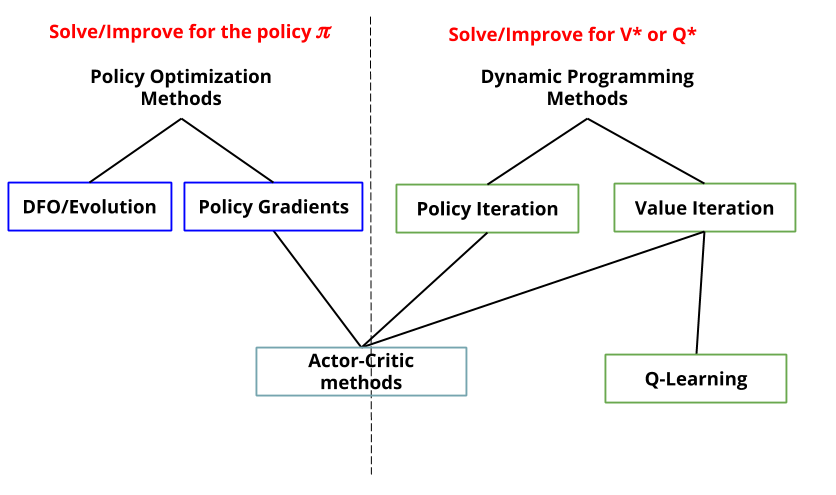
\includegraphics[width=0.9\textwidth]{./chapters/chapter_2/imgs/img_rl_methods.png}
        \caption{RL solution methods landspace. \textbf{Value-based methods} (right) solve for the policy 
                 indirectly, whereas \textbf{Policy-based methods} (left) solve for the policy directly.}
        \label{fig:ch2_rl_policies_differences}
    \end{figure}
}

\newcommand{\figRlPolicyGradientsIntuition}{
    \begin{figure}[!b]
        \centering
        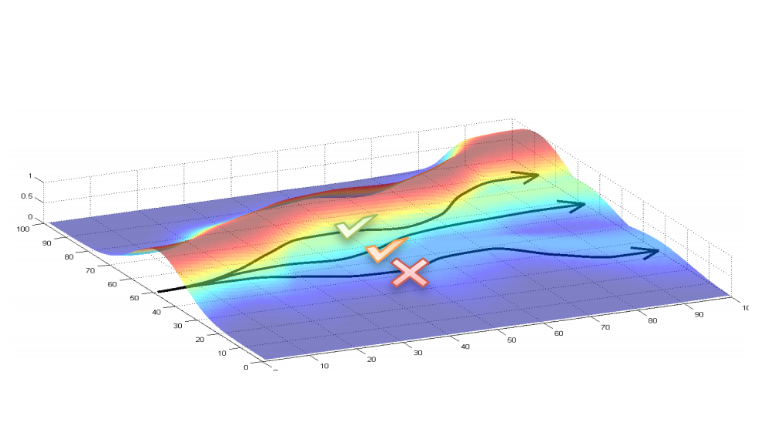
\includegraphics[width=0.8\textwidth]{./chapters/chapter_2/imgs/img_rl_pg_intuition.png}
        \caption{Intuition behind Policy Gradients. Actions that yield good trajectories are encouraged}
        \label{fig:ch2_rl_pg_intuition}
    \end{figure}
}

\newcommand{\figRlPolicyParametrization}{
    \begin{figure}
        \centering
        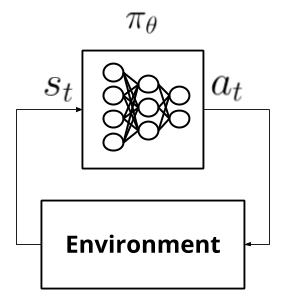
\includegraphics[width=0.3\textwidth]{./chapters/chapter_2/imgs/img_policy_parametrization.png}
        \caption{Parametrization of a policy $\pi$ using a Neural Network}
        \label{fig:ch2_rl_policy_parametrization}
    \end{figure}
}

\newcommand{\figALEgames}{
    \begin{figure}[H]
        \centering
        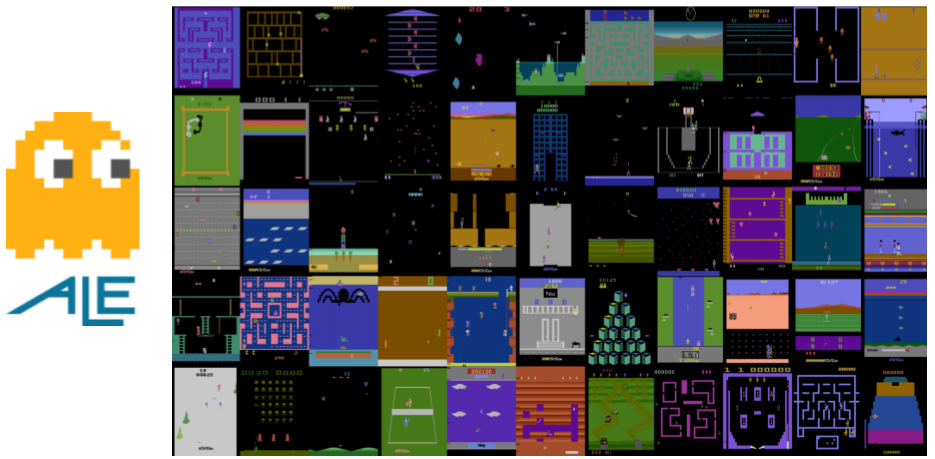
\includegraphics[width=0.6\textwidth]{./chapters/chapter_2/imgs/img_atari_learning_environment.png}
        \caption{Games in the Atari Learning Environment.}
        \label{fig:ch2_ale_games}
    \end{figure}
}

\newcommand{\figOpenAIEnvs}{
    \begin{figure}[H]
        \centering
        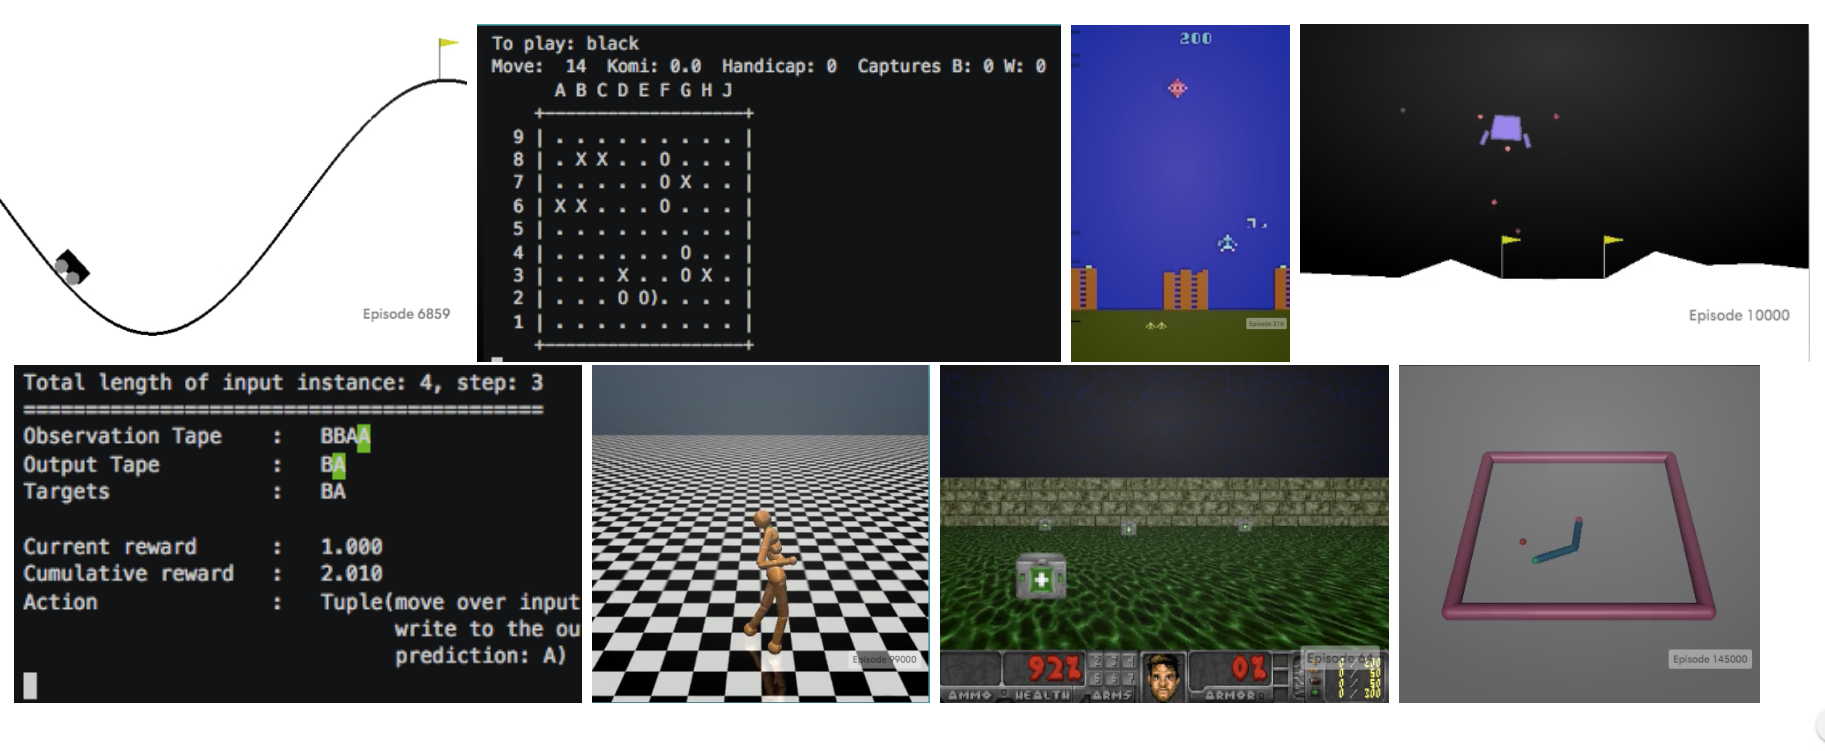
\includegraphics[width=0.9\textwidth]{./chapters/chapter_2/imgs/img_openai_gym_envs.png}
        \caption{Environments in OpenAI Gym.}
        \label{fig:ch2_gym_envs}
    \end{figure}
}

\newcommand{\figDeepmindLabEnvs}{
    \begin{figure}[H]
        \centering
        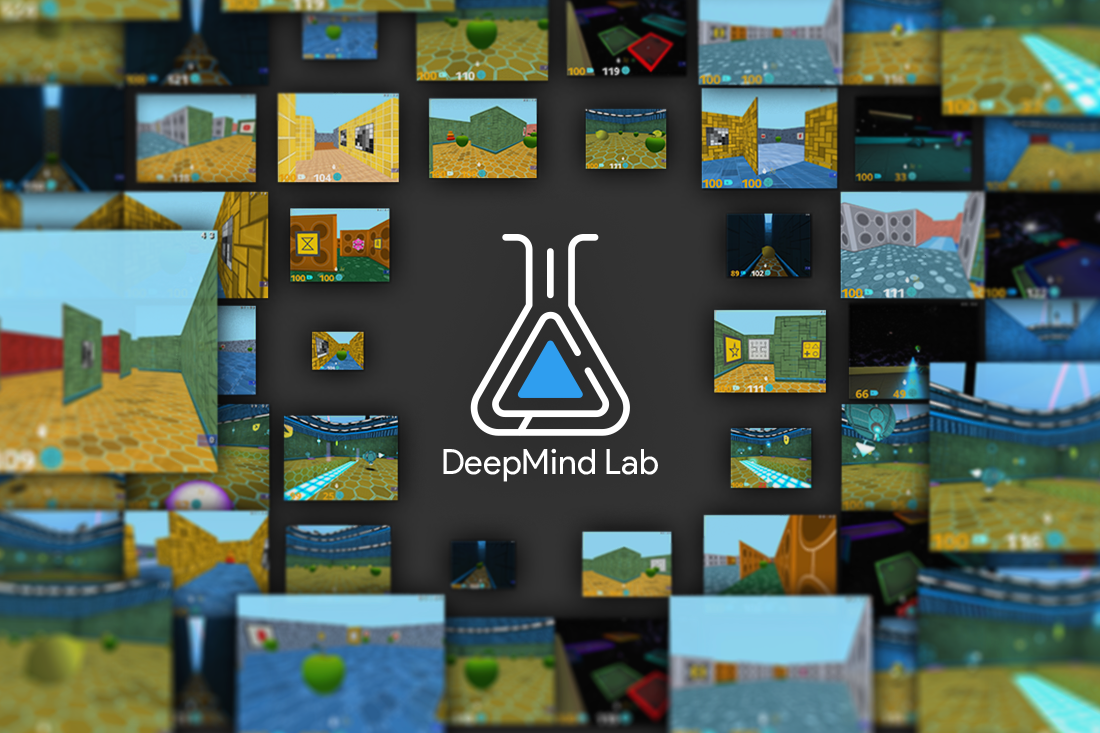
\includegraphics[width=0.7\textwidth]{./chapters/chapter_2/imgs/img_deepmind_lab.png}
        \caption{Environments in Deepmind Lab}
        \label{fig:ch2_deepmind_lab}
    \end{figure}
}

In this chapter we we will give an overview of the core concepts needed to
understand the following chapters in this document. These include:


\begin{itemize}
    \item A brief overview of the field of \textbf{Deep Reinforcement Learning}, where
          we describe some concepts of Reinforcement Learning, Deep Learning, and Deep
          Reinforcement Learning.
    \item An overview of \textbf{learning environments}, which are a key component of
          the Reinforcement Learning framework. We analyze why are they important 
          and some examples used in current Deep Reinforcement Learning research.
    \item A more specific overview of \textbf{learning environments for robot locomotion}, 
          what are their components, and some concepts about their design. This is
          intended for the first half of the proposal which consists of making this type
          of learning environments.
\end{itemize}


\section{Deep Reinforcement Learning}

At a very high level Deep Reinforcement Learning (DeepRL) could be thought as a combination 
of current Deep Learning (DL) models and techniques, with the framework of Reinforcement 
Learning (RL), to solve complex RL problems. This combination has given impressive 
results over the past few years, like being able to play a suite of atari games \citep{DQNAtari}, 
beating the world Go champion \citep{AlphaGo}, making simulated characters develop locomotion
skills [\citeauthor{DeepmindEmergenceLocomotion},\citeauthor{DeepTerrainRL},\citeauthor{DeepMimic}], 
and being able to learn manipulation and locomotion tasks in 
real-world robotics platforms [\citeauthor{EndToEndVisuoMotorPolicies},\citeauthor{ScalableDeepRL},\citeauthor{GoogleBrainSim2Real}],
just to name a few.

\figdrlsamplesFirst

\figdrlsamplesSecond

\figdrlsamplesThird

\todo{Parece un poco informal usar Let's start, usa otra frase o simplemente sácala} 
In the followings subsections we define Reinforcement Learning, present classic solutions methods, and then
discuss how Deep Learning fits into this framework by providing a way to capture representation
in the context of function approximation.

\subsection{Reinforcement Learning}

\todo{En toda esta subsección no vi una referencia, por lo menos indicar en que autor te basaste para escribirla}
Reinforcement Learning is an overloaded term that encloses both a \textbf{learning paradign}
and the \textbf{algorithms} that solve problems in this framework. Reinforcement Learning \todo{mejor decir directamente que is a learning paradigm like}
is a learning paradigm, like supervised and unsupervised learning, but unlike these other paradigms \todo{Aqui colocar un punto y comenzar con Unlike learning from ... en vez de with the difference...} 
in Reinforcement Learning an agent has to learn by interactions with an environment.

In Figure ~\ref{fig:ch2_rlloop} we show the Agent-Environment interaction loop. This represents
the way an agent in a certain \textbf{state} $S_{t}$ (a certain modeled configuration) interacts 
with its environments by means of some \textbf{action} $A_{t}$, and models how the environment 
responds by giving the agent a \textbf{reward} $R_{t+1}$ (basically a score for its interaction) 
and a \textbf{new state} $S_{t+1}$ (obtained from the environment dynamics).

\figrlloop

We can formalize this setting with Markov Decision Processes (MDPs)\todo{referencia}, which is a framework
that we can use to model sequential decision making problems with uncertainties.

\begin{definition}
    A Markov Decision Process (MDP) is a 5-tuple of the following components:
    \begin{itemize}
        \item A set of states $s \in S$
        \item A set of actions $a \in A$
        \item A transition model $T(s',s,a) = P(s'|s,a)$
        \item A reward function $R(s',s,a)$
        \item A discount factor $\gamma$
    \end{itemize}
\end{definition}

We have already discussed \todo{discussed} some of the components of an MDP (state, action, reward).
The remaining components consist of: a transition model of the environment, $P(s'|s,a)$
which basically models the environment's dynamics into a single conditional probability
distribution, and a discount factor $\gamma$ used to take into account that rewards in the future might have \todo{that .. that no suena muy bien}
less importance than rewards now (discounting like when dealing with money). Some examples 
of problems in RL formulated in the MDP framework are shown in Figure ~\ref{fig:ch2_mdps_samples}.

\figMdpSamples

The objective of the agent is to maximize the expected sum of rewards it gets from
its interaction with the environment. To achieve this it has to come up with a
way to select the appropriate actions in a given situation, which in this case is given
by the state of the agent. To formalize this, let's \todo{usa algo más formal} define some extra concepts:

\begin{itemize}
    \item \textbf{Returns}, which is a more compact notation to express the sum of rewards.
    \item \textbf{Policies}, which are the way an agent picks its actions, meaning they
          are the solution to our RL problem.
\end{itemize}

\newpage

\begin{definition}
    The return $G_{t}$ is defined as the sum of rewards an agent gets from its
    interactions starting at timestep $t$.
    \begin{equation}
        G_{t} = \sum_{k=0}^{\infty} \gamma^{k} R_{t+k+1}
    \end{equation}
\end{definition}

\begin{definition}
    A deterministic policy $\pi(s)$ is defined as a mapping between states $s \in S$
    to action $a \in A$.
    \begin{equation}
        \pi : S \rightarrow A
    \end{equation}
\end{definition}

\begin{definition}
    An stochastic policy $\pi(a|s)$ is defined as a conditional probability distribution over
    states $s \in S$ of a certain action $a \in A$.
    \begin{equation}
        \pi : S \times A \rightarrow [0,1]
    \end{equation}
\end{definition}

\figRlPolicies

Figure ~\ref{fig:ch2_rl_policies_differences} shows the differences between an stochastic policy and a deterministic
policy. We can reformulate the objective of the agent into the following: \textit{An agent's objective
in the RL setup is to maximize the expected return $\mathbb{E} \lbrace G_{t} \rbrace$ it
can get from its interactions with the environment by finding the best policy $\pi$, which
we call optimal policy, and denote by $\pi^{*}$}

\begin{equation}
    \pi^{*} = \arg \max_{\pi} \mathbb{E}_{\pi} \lbrace G_{t} \rbrace
\end{equation}

\subsection{Solution methods}

\figRlMethodsLandspace

To solve an MDP there are various methods that can be used. Most of them are
summarized in the categories shown in Figure ~\ref{fig:ch2_rl_policies_differences}. These include:

\begin{itemize}
    \item \textbf{Value based methods}, which try to solve for some auxiliary
          functions, called \textit{State-value} and \textit{Action-value} functions
          and then extract the solution directly. These methods make use of the Bellman
          Backups iteratively to find a solution that satisfies the Bellman Equations\todo{referencia}.
    \item \textbf{Policy based methods}, which solve for\todo{ quitar} the policy directly. These methods
          make use of some parametrization of the policy via some function approximator
          (like a Neural Network), and then search for the parameters of this policy
          by optimizing the expected return.
\end{itemize}

Most of the current methods used are Policy based methods, specially in the context
of robot locomotion \todo{referencia}. In the following section we will cover some concepts used when
using policy based methods. 

We will also focus specially in \textbf{model-free} methods,
which don't require information of the transition model of the environment. Most of the
literature deals with these type of methods, although because of this assumption these
methods are usually very sample inefficient (They need a lot of interaction samples to be
able to learn).

\subsection{Policy Optimization}

As described earlier, policy based methods try to solve for the parameters $\theta$
of a parametrized policy $\pi_{\theta}$ such that this policy maximizes the expected
return the agent gets from its interactions with the environment.

\begin{equation}
    \theta = \arg \max_\theta \mathbb{E}_{\pi_{\theta}} \lbrace G_{t} \rbrace
\end{equation}

One way to solve this optimization problem is to apply Derivative Free Optimization
methods, like evolutionary algorithms \todo{referencia}. These black box optimization methods would
search for the right set of parameters that satisfy the objective we are requesting.

We will focus in Gradient based optimization methods, which make use of gradient
ascent to search for the right set of parameters. The kind of gradient used in this
case is an estimate of the gradient of this\todo{its?} expectation objective, which we can sample
using sample trajectories of interaction, and then use it with an optimizer like
SGD. Let's introduce some extra concepts and then present this gradient estimate,
and the base form of the Policy Gradients algorithms.

\begin{definition}
    A trajectory $\tau$ is defined as a consecutive sequence of states, actions 
    and rewards experienced by an agent over its interactions with the environment.
    \begin{equation}
        \tau = \lbrace s_{0},a_{0},r_{1},s_{1},a_{1},r_{2},\hdots,s_{H-1},a_{H-1},r_{H} \rbrace
    \end{equation}
\end{definition}

\begin{definition}
    We define the return over a trajectory $G(\tau)$ as the discounted sum of
    rewards obtained in that trajectory.
    \begin{equation}
        G(\tau) = \sum_{t=0}^{H} \gamma^{t} r_{t+1}
    \end{equation}
\end{definition}

We  can then reformulate the objective we want to optimize for using this new notation.
Recall that the agent tries to maximize its expected return, so we can define this as
an objective $J$ that depends on the parameters of our policy as follows:

\begin{equation}
    J(\theta) = \mathbb{E}_{\tau \sim p(\tau;\theta)}[G(\tau)] = \sum_{\tau} p(\tau;\theta) G(\tau)
\end{equation}

Where $p(\tau;\theta)$ is a probability distribution of trajectories, induced by
the parameters of our policy $\theta$ (recall that the agent sees what its policy allows).
We can then optimize for the parameters $\theta$ by computing the gradient of this
objective function. However, directly trying to compute the gradient of this expectation
is intractable, thus we make use of a mathematical trick (REINFORCE trick) to get an estimate of this gradient \citep{PGSutton}. \todo{en vez de so, usa thus, es más formal}

\begin{theorem}
    For any differentiable policy $\pi_{\theta}(a|s)$, the gradient of the
    objective function $J(\theta) = \sum_{\tau} p(\tau;\theta) G(\tau)$ 
    can be computed using the following policy gradient.
    \begin{equation}
        \nabla_{\theta} J(\theta) = \mathbb{E}_{\pi_{\theta}} \lbrace G(\tau) \nabla_{\theta} \log \pi_{\theta} \rbrace
    \end{equation}
\end{theorem}

The resulting expression from the previous theorem needs no information of the model.
The only requirement is for the policy to be differentiable. We can compute this expected
gradient by using samples, and then apply gradient ascent in the parameters space to optimize 
the parameters $\theta$ of our policy.

The intuition of this algorithm is that it is increasing the probability of selecting
the actions that yielded good results (from the trajectories that gave good returns), 
and decreasing the probability of selecting the actions that yielded bad results. This
is shown in the Figure ~\ref{fig:ch2_rl_pg_intuition}.

\figRlPolicyGradientsIntuition

\subsection{Deep Learning and RL}
\todo{toda esta subsection no tiene referencias}
As already explained earlier, we make use of function approximation to parameterize
some component of our RL setup. In value based methods we usually parameterize the
Action-value function as $Q_{\theta}$, and in policy based methods we parameterize
the policy as $\pi_{\theta}$. These parametrization can be made by using various
function approximators \todo{revisa si existe esta palabra, creo que seria mejor approximations}, like \textit{linear models}, \textit{fourier basis}, 
\textit{decision trees}, \textit{radial basis functions}, etc..

Deep learning is used in this context to provide function approximators via Deep
Neural Networks, as shown in Figure ~\ref{fig:ch2_rl_policy_parametrization}. 
In this case, our $\theta$ parameters are the weights of a neural network used 
to represent our policy. We can use the machinery from before (Policy Gradients)
to optimize for the parameters of our network.

\figRlPolicyParametrization

The term Deep Reinforcement Learning refers to this approach of using Deep Neural Networks
as function approximators in the RL framework. The key difference behind this approach
and previous works that used different function approximators is that in previous works
the use of function approximators was decoupled from the representation given to the mode.
The representation was given by features that where hand engineered by the researcher, and then
combined with the function approximator chosen for the task. The approach that DeepRL follows is 
different in the sense that we learn the representation via the Deep models we use as function approximators. \todo{se esta usando excesivamente la palabra approximator en este parrafo}

\section{Simulated Learning Environments}

One key component of the RL framework (and one that seems to be trivial) is the learning
environment itself. This learning environment is used by the agent to get samples of
experience and then learn using the machinery explained in previous sections. It is analogous
to the role that a dataset plays in Supervised Learning.

These learning environments are usually simulations of some RL tasks that we want an
agent to learn. This simulated nature of the environment makes it easy to grab as much 
experience as needed, and because the environment is a simulation we can usually
speed up the process and take huge amounts of experience for our learning algorithms.

A learning environment is usually designed around the agent interaction loop mentioned
at the beginning of this chapter. This defines the basic API that such an environment
has to provide:

\begin{itemize}
    \item A representation for the \textbf{actions} to take in the simulation.
    \item A \textbf{reward} to give to the agent because of the action taken.
    \item A \textbf{state} (or observation) to give to the agent because of the action taken.
\end{itemize}

Some learning environments have become benchmarks for testing DeepRL algorithms, and
are widely used because of this standarization. Just to name a few:

\begin{itemize}

    \item \textbf{The Arcade Learning Environment} (ALE) \citep{BellemareALE}, which provides a suite
           of Atari games to be used as DeepRL benchmarks. This was used in the DQN
           agent made by Deepmind \citep{DQNAtari}, which started the interest in DeepRL.
           The core of the environment is an emulator for the Atari 2600 games, and
           it has functionality to access registers from the emulated game, and return
           this state. Some of these registers are loaded with the score of the game
           and can be retrieved to be exposed to the user. The observations consist
           of frames from the rendered game, which are also exposed to the user. The actions
           are mapped into the appropriate register that the emulator expects in order
           to apply the joystick controls in the game.

           \figALEgames

    \item \textbf{OpenAI Gym} \citep{Gym}. This toolkit provides various learning environments
           as benchmarks for RL algorithms. It contains simple benchmarks, starting from simple
           toy problems like gridworlds, and it also contains more complicated benchmarks like
           games (like Atari 2600 games), robotics manipulation tasks and also various
           robotics locomotion benchmarks, which we will cover in the next section.

           \figOpenAIEnvs

    \item \textbf{Deepmind Lab} \citep{DeepmindLab}, which is a 3D learning environment built on top
           of the Quake game engine, from \textit{Id Software}. It provides various challenging
           environments like mazes, multi-agent setups, etc. The actions are mapped to a discrete
           set of actions that the original game engine supported, and the observations consists
           mainly of the camera frames from the rendered game.

           \figDeepmindLabEnvs

\end{itemize}

\section{Simulated Environments for Robot Locomotion}

In this section we discuss about learning environments for robot locomotion tasks.
These make use of different components to provide the simulation required for the desired
tasks (like walking, running, standing, etc.). The main components we will use
to describe these environments are the underlying \textbf{physics engine} used for the simulations, 
the internal agent representation of an agent by using \textbf{kinematic trees}, and the
the underlying representation of the agent actions we can apply by using an appropriate \textbf{actuation model}.

\subsection{Physics Engines}

The physics engine is the component in charge of simulating the environment by doing the
required collision checking and applying the dynamics to the simulated objects. These
physics engines vary according to the application needed and the methods used for solving
the underlying problems required for the simulations. A brief summary of the steps involved are
shown in Figure ~\ref{fig:ch2_physics_engines_loop}.

\figPhysicsEngineLoop

Different physics engines make changes in different parts of this general pipeline.
The changes are made based on some trade-offs that depend on the application. That's
why some engines are more suited for applications like games (by reducing accuracy for speed)
and some other are more suited for robotics applications (by being more accurate in 
contact calculations, actuation models, etc.). Some available physics engines are 
listed below:

\begin{itemize}
    \item \textbf{MuJoCo} \citep{MuJoCo}, developed by Emo Todorov, is a recent physics engine
          used for robotics applications, and widely used for RL locomotion benchmarks through
          various python packages made by various researchers, like Deepmind's controlsuite \citep{Controlsuite},
          Berkeley's Rllab, OpenAI's mujoco-py, etc. This engine is closed source and it
          requires a license for continuous use.

    \item \textbf{Bullet} \citep{Bullet}, developed by Erwin Cowmans, is a very popular opensouce
          physics engine. It provides both C/C++ and Python APIs, and it's been used in packages
          like OpenAI's Roboschool \citep{Roboschool}, and in research in \cite{DeepTerrainRL} and \cite{DeepMimic}.

    \item \textbf{PhysX} \citep{PhysX}, developed by NVIDIA, is a physics engine used
          mostly in games, and integrated into game engines like \citeauthor{Unity} and \citeauthor{Unreal}.
          It has recently been released as open source, and version 4.0 has new features
          that allow to simulate robotics applications more accurately.

    \item \textbf{FleX} \citep{FleX}, developed also by NVIDIA, is a GPU particle-physics engine,
          it uses position-based dynamics (unlike the others which are force-based), which is
          more visually pleasing, but not accurate to simulate the real world. The advantage is
          that is possible to simulate large scenes easily and with very few compute resources.
          For example, in \cite{GpuSim} the authors (also from NVIDIA) developed a simulator based on
          this physics engine, and they show that they can simulate large scene with hundreds of
          agents.
\end{itemize}

\subsection{Kinematic trees}

A kinematic tree is the internal data structure used to hold the information of
an agent composed of links (bodies) and joints (constraints). Each node in the 
tree represents a link of the agent, and it connects to other nodes according to
the joints shared between these nodes. An example of a kinematic tree is shown in
Figure ~\ref{fig:ch2_kinematic_tree_representation}. 

This data structure is usually used for character animation, because by traversing 
the tree we can propagate the world positions and orientations of each body. In the
case of robot locomotion is used internally by the engine to do internal calculations,
some of them related to computing forces and torques using the Featherstone algorithm \citep{Featherstone},
which allows to compute these forces using $O(n)$ cost, where $n$ is the number of
links in the kinematic tree.

\figKinTreeRepresentation

\subsection{Actuation models}

An actuation model refers to how the simulation handles an input received in an actuator
of the simulated agent. Depending on the type of actuation model, a given agent
can behave very different given the same input. Some actuation models are listed below:

\begin{itemize}
    \item \textbf{Torques}, which are applied directly to the actuated joints.
    \item \textbf{Target positions}, which are requested angles for the actuated joints,
          and translated into torques via PD controllers.
    \item \textbf{Target velocities}, which are requested velocities for the actuated joints,
          and translated into torques via a P controller over the velocities.
    \item \textbf{Muscle activations}, which are requested activations to a set of tendons
          related to an actuated joint.
\end{itemize}

For more details in actuation models, see \cite{ActuationChoice}. Some physics engines don't support 
various of this actuation models, leaving the user with the responsibility to implement
these models using the primitives provided, which usually consist in torques (like the authors
of \citep{DeepmindEmergenceLocomotion} did in its implementation). Figure ~\ref{fig:ch2_actuation_models} 
shows these actuation models (adapted from \cite{ActuationChoice}).

\figActuationModels

\todo{deberias colocar una seccion de consideraciones finales para hacer un pequeño resumen del capitulo presentado y presentar lo que será visto en el siguiente de forma breve}
